% !TEX root = main.tex
% !TEX encoding = Windows Latin 1
% !TEX TS-program = pdflatex
% 
%
% Plantilla para las tesis de ingenieria de la Universidad de los Andes
% 2012/07/27, v.1.9

% Para las opciones de clase, ver la documentacion
\documentclass[publish,english]{tui}
\checklanguage

%\include{personal} % Incluya aqui el archivo con su comandos personales y los paquetes adicionales que quiera cargar.

% !TEX root = main.tex
% !TEX encoding = Windows Latin 1
% !TEX TS-program = pdflatex
% 
% Archivo de particion de palabras

\hyphenation{%
  % Introduzca aqui las palabras que requieran division especial, separadas por espacios.
  % No se pueden usar acentos en estas palabras (a menos que se use codificacion UTF8).
  
}


\endinput  % Excepciones de guiones (editar archivo)


% --------------------------------------------
% En caso de NO usar indice analitico (no recomendado),
% comentar esta seccion:
\makeatletter
  \iftui@draft\relax
    \else\makeindex % indice analitico
  \fi
\makeatother

%----------------------------------------------

\begin{document}% =========================================
\setupeverything
\frontmatter % Los preliminares de la tesis
\pagestyle{empty}

% !TEX root = main.tex
% !TEX encoding = Windows Latin 1
% !TEX TS-program = pdflatex
%
% portada.tex (portadilla y portada de la tesis)

% +++++++++++++++++++++++ Portadilla +++++++++++++++++++++++++++++
%
\pagestyle{empty}
\dosenblanco

% Portadilla
\begin{center}
  \scshape%
  % Aqui va el titulo de la tesis----------------------------------
  Este es el t\'{i}tulo \\
  de la tesis doctoral \\
  % ---------------------------------------------------------------
\end{center}

\cleardoublepage

% +++++++++++++++++++++++ Portada +++++++++++++++++++++++++++++
%
\begin{center}
{%
  \LARGE\scshape\bfseries%
  % Aqui va el titulo de la tesis ---------------------------
  Este es el t\'{i}tulo \\ [6pt]
  de la tesis doctoral \\ [6pt]
  % ---------------------------------------------------------
}

\vfill

{
 \large\scshape%
  A dissertation\\
  by\\
  % Aqui va el autor de la tesis-----------------------------
  Este es el autor de la tesis
  % ---------------------------------------------------------
}

\vfill

{%
  % Datos de la Universidad, el titulo, etc. ------------------
  {\normalfont Submitted to the School of Engineering of the}\\[3pt]
  {\large\scshape Universidad de los Andes}\\[3pt]
  {\normalfont in partial fulfillment for the requirements for the Degree of}\\[3pt]
  {\large\scshape Doctor in Engineering}
  % -------------------------------------------------------------
}

\vfill

%----------------------- No tocar este codigo ----------------------
\makeatletter
  \iftui@spanish
    {\scshape Aprobada por:}
  \else
    {\scshape Approved by:}
  \fi
\makeatother
% ------------------------------------------------------------------


% Llenar esta informacion ------------------------------------------
\begin{tabbing}
  \hspace{6.5cm}\=\kill
  \hspace{1cm}Committee Chair:    \> {\itshape Dr. . . . } \\
  \hspace{1cm}Committee Members:  \> {\itshape Prof. . . . } \\
  			    											 \> {\itshape Prof. . . . } \\
                                  \> {\itshape Prof. Dr. . . . } \\
                                  \> {\itshape Prof. Dr. . . . } \\
                                  \> {\itshape Prof. Dr. . . . } \\
                                  \> {\itshape Prof. Dr. . . . } \\
                                  \> {\itshape Prof. Dr. . . . } \\
                                  
  \hspace{1cm}Dean School of Engineering: \> {\itshape Dr. Alain Gauthier} \\
  \hspace{1cm}Assistant Dean: \> {\itshape Dr. Rubby Casallas}
\end{tabbing}
% --------------------------------------------------------------------

\vfill

{%
  \normalsize\scshape
  % Fecha y area --------------------------------------------------
  February 2011\\
  {\scshape%
  Field: Ingenier\'{i}a de Sistemas y Computaci\'{o}n
  % ---------------------------------------------------------------
  }
}

\end{center}



% Fin de portada.tex
\endinput  % Portadilla y portada (editar archivo)

\makeatletter
\iftui@publish
  % !TEX root = main.tex
% !TEX encoding = Windows Latin 1
% !TEX TS-program = pdflatex
%
% plegal.tex (Pagina legal de la tesis)


\hbox{}\thispagestyle{empty}

\vspace*{-2cm}
\begin{center}
\noindent
\fbox{\parbox{\textwidth}{%
\scriptsize
 \vspace*{3cm}

 [Informaci{\'o}n p{\'a}gina legal]

 \vspace*{3cm}
}}

\end{center}

\vfill


{%
\parindent=0pt
\scriptsize

Primera edici{\'o}n:  Febrero de 2010\\

\copyright\ [Nombre del autor]\\
\url{email@del.autor}

\medskip

\copyright\ Universidad de los Andes, Facultad de Ingenier\'{\i}a\\
\phantom{\copyright\ }Departamento de Ingenier\'{\i}a * * * * * * * * * * * * \\

\bigskip

Ediciones Uniandes\\ Carrera 1\textsuperscript{a} No. 19-27. Edificio AU 6\\
Bogot{\'a} \textsc{DC}, Colombia\\
Tel{\'e}fono: 339 49 49 / 339 49 99. Ext: 2133. Fax: ext. 2158\\
\url{http://libreria.uniandes.edu.co}\\
\url{infeduni@uniandes.edu.co}

\bigskip

ISBN: [N{\'u}mero del ISBN]

\bigskip

Correcci{\'o}n de estilo en ingl{\'e}s: xxxxxxxxxxxxxx

\bigskip

Dise{\~n}o de car{\'a}tula: xxxxxxxxxxxxxx

\bigskip

Dise{\~n}o de colecci{\'o}n: Nicol{\'a}s Vaughan

\bigskip

Impresi{\'o}n: [Nombre editorial] \\ \
[Direcci{\'o}n] \\ \
Bogot{\'a} \textsc{DC}, Colombia

}

\vfill

\begin{tiny}
\begin{flushleft}
\noindent  Impreso en Colombia -- Printed in Colombia\\

\noindent Todos los derechos reservados. Esta publicaci{\'o}n no puede
ser reproducida ni en su todo ni en sus partes, ni registrada en o
trasmitida por un sistema de recuperaci{\'o}n de informaci{\'o}n, en ninguna
forma ni por ning{\'u}n medio sea mec{\'a}nico, fotoqu\'{\i}mico, electr{\'o}nico,
magn{\'e}tico, electro-{\'o}ptico, por fotocopia o cualquier otro, sin el
permiso previo por escrito de la editorial.
\end{flushleft}
\end{tiny}

% Fin de plegal.tex
\endinput  % Pagina legal (editar archivo)
  % !TEX root = main.tex
% !TEX encoding = Windows Latin 1
% !TEX TS-program = pdflatex
%
% Archivo: coleccion.tex (Descripcion de la coleccion de tesis)

% ------------  Importante: No editar este archivo ----------------------------

\selectlanguage{spanish}
\chapter*{Descripci{\'o}n de la colecci{\'o}n}
\thispagestyle{empty}
\noindent
Esta colecci{\'o}n re{\'u}ne los mejores trabajos de grado de maestr\'{\i}a y de doctorado de la Facultad de Ingenier\'{\i}a de la Universidad de los Andes. Con el {\'a}nimo de divulgar estos resultados de nuestros grupos de investigaci{\'o}n, la Facultad los pone a disposici{\'o}n de la comunidad acad{\'e}mica.

\bigskip

\noindent
Decano, Alain Gauthier Sellier; Vicedecana de Posgrado e Investigaci{\'o}n, Rubby Casallas Guti{\'e}rrez; Vicedecano de Pregrado, Rafael G{\'o}mez D\'{\i}az; Vicedecano para el Sector Externo, Gonzalo Torres Cadena; Secretaria General, Claudia C{\'a}rdenas Guti{\'e}rrez; Directores de Departamento: de Ingenier\'{\i}a Civil y Ambiental, Arcesio Lizcano Pel{\'a}ez; de El{\'e}ctrica y Electr{\'o}nica, Roberto Bustamante Miller; de Industrial, Roberto Zarama Urdaneta; de Mec{\'a}ni\-ca, {\'E}dgar Alejandro Mara{\~n}{\'o}n Le{\'o}n; de Qu\'{\i}mica, {\'O}scar {\'A}lvarez Solano; de Sistemas y Computaci{\'o}n, Jorge Alberto Villalobos Salcedo.



\checklanguage
% Fin archivo coleccion.tex
\endinput 
 % Descripcion coleccion tesis (no editar archivo)
  \else\relax\fi
\makeatother

\cleardoublepage

% !TEX root = main.tex
% !TEX encoding = Windows Latin 1
% !TEX TS-program = pdflatex
% 
% agradec.tex (Agradecimientos de la tesis)

\thispagestyle{empty}

\ 

\vspace*{2cm}

{
\flushright\itshape

****,\\
****,\\
****.\\

}


\vfill




% Fin de dedicat.tex
\endinput  % Dedicatoria (opcional) (editar archivo)
% !TEX root = main.tex
% !TEX encoding = Windows Latin 1
% !TEX TS-program = pdflatex
% 
% agradec.tex (Agradecimientos de la tesis)

\Agradecimientos
\noindent








% Fin de agradec.tex
\endinput  % Agradecimientos (editar archivo)
% !TEX root = main.tex
% !TEX encoding = Windows Latin 1
% !TEX TS-program = pdflatex
% 
% Archivo: abstract.tex (en ingles)


\chapter{Abstract} % No cambiar el titulo
\selectlanguage{english}
\noindent
Duis tristique sollicitudin leo nec consequat. Praesent et dui convallis velit tincidunt fermentum. Mauris cursus purus at sem viverra sed imperdiet sapien imperdiet. Aliquam mattis, elit eget rutrum vulputate, tortor sem pulvinar justo, sit amet mollis felis sem at nibh. Donec malesuada, neque id interdum eleifend, arcu augue porta elit, nec tristique libero metus at massa. Fusce fringilla laoreet rhoncus. Suspendisse potenti. Phasellus dignissim sodales mauris at pharetra. Donec gravida fringilla velit ac rutrum.

Curabitur ornare lectus id diam molestie eu imperdiet nulla tempus. Maecenas vestibulum enim et dui ornare blandit. Vivamus fermentum faucibus viverra. Maecenas at justo sapien. Aenean rhoncus augue mattis purus rhoncus venenatis. Suspendisse metus felis, porttitor in varius in, vulputate at tortor. Aliquam molestie, turpis et malesuada porta, tortor sapien pharetra sapien, ac rhoncus quam dolor a sapien. Pellentesque varius laoreet enim ut auctor. Nullam nec ultricies nisi. Nullam porta lectus et ante consectetur posuere.

Duis tristique sollicitudin leo nec consequat. Praesent et dui convallis velit tincidunt fermentum. Mauris cursus purus at sem viverra sed imperdiet sapien imperdiet. Aliquam mattis, elit eget rutrum vulputate, tortor sem pulvinar justo, sit amet mollis felis sem at nibh. Donec malesuada, neque id interdum eleifend, arcu augue porta elit, nec tristique libero metus at massa. Fusce fringilla laoreet rhoncus. Suspendisse potenti. Phasellus dignissim sodales mauris at pharetra. Donec gravida fringilla velit ac rutrum.

Duis tristique sollicitudin leo nec consequat. Praesent et dui convallis velit tincidunt fermentum. Mauris cursus purus at sem viverra sed imperdiet sapien imperdiet. Aliquam mattis, elit eget rutrum vulputate, tortor sem pulvinar justo, sit amet mollis felis sem at nibh. Donec malesuada, neque id interdum eleifend, arcu augue porta elit, nec tristique libero metus at massa. Fusce fringilla laoreet rhoncus. Suspendisse potenti. Phasellus dignissim sodales mauris at pharetra. Donec gravida fringilla velit ac rutrum.

Curabitur ornare lectus id diam molestie eu imperdiet nulla tempus. Maecenas vestibulum enim et dui ornare blandit. Vivamus fermentum faucibus viverra. Maecenas at justo sapien. Aenean rhoncus augue mattis purus rhoncus venenatis. Suspendisse metus felis, porttitor in varius in, vulputate at tortor. Aliquam molestie, turpis et malesuada porta, tortor sapien pharetra sapien, ac rhoncus quam dolor a sapien. Pellentesque varius laoreet enim ut auctor. Nullam nec ultricies nisi. Nullam porta lectus et ante consectetur posuere.

Duis tristique sollicitudin leo nec consequat. Praesent et dui convallis velit tincidunt fermentum. Mauris cursus purus at sem viverra sed imperdiet sapien imperdiet. Aliquam mattis, elit eget rutrum vulputate, tortor sem pulvinar justo, sit amet mollis felis sem at nibh. Donec malesuada, neque id interdum eleifend, arcu augue porta elit, nec tristique libero metus at massa. Fusce fringilla laoreet rhoncus. Suspendisse potenti. Phasellus dignissim sodales mauris at pharetra. Donec gravida fringilla velit ac rutrum.

\bigskip
\noindent
\textit{Key words:} first word; second word; third word.
% Separar palabras con punto-y-comas.

\checklanguage
% Fin archivo abstract.tex
\endinput  % Resumen ingles (editar archivo)
% !TEX root = main.tex
% !TEX encoding = Windows Latin 1
% !TEX TS-program = pdflatex
%
% Archivo: resumen.tex (en espanol)


\chapter{Resumen} % No cambiar el titulo
\selectlanguage{spanish}
\noindent
Duis tristique sollicitudin leo nec consequat. Praesent et dui convallis velit tincidunt fermentum. Mauris cursus purus at sem viverra sed imperdiet sapien imperdiet. Aliquam mattis, elit eget rutrum vulputate, tortor sem pulvinar justo, sit amet mollis felis sem at nibh. Donec malesuada, neque id interdum eleifend, arcu augue porta elit, nec tristique libero metus at massa. Fusce fringilla laoreet rhoncus. Suspendisse potenti. Phasellus dignissim sodales mauris at pharetra. Donec gravida fringilla velit ac rutrum.

Curabitur ornare lectus id diam molestie eu imperdiet nulla tempus. Maecenas vestibulum enim et dui ornare blandit. Vivamus fermentum faucibus viverra. Maecenas at justo sapien. Aenean rhoncus augue mattis purus rhoncus venenatis. Suspendisse metus felis, porttitor in varius in, vulputate at tortor. Aliquam molestie, turpis et malesuada porta, tortor sapien pharetra sapien, ac rhoncus quam dolor a sapien. Pellentesque varius laoreet enim ut auctor. Nullam nec ultricies nisi. Nullam porta lectus et ante consectetur posuere.


Curabitur ornare lectus id diam molestie eu imperdiet nulla tempus. Maecenas vestibulum enim et dui ornare blandit. Vivamus fermentum faucibus viverra. Maecenas at justo sapien. Aenean rhoncus augue mattis purus rhoncus venenatis. Suspendisse metus felis, porttitor in varius in, vulputate at tortor. Aliquam molestie, turpis et malesuada porta, tortor sapien pharetra sapien, ac rhoncus quam dolor a sapien. Pellentesque varius laoreet enim ut auctor. Nullam nec ultricies nisi. Nullam porta lectus et ante consectetur posuere.


\bigskip
\noindent
\textit{Palabras clave:} palabra uno; palabra dos; palabra tres.

\checklanguage
% Fin archivo resumen.tex
\endinput  % Resumen espanol (editar archivo)


% Tabla de contenido, dependiendo del idioma
\tuitableofcontents

\cleardoublepage

\listoftables  % En caso de que haya tablas --------------
% (comentar en caso contrario)

\cleardoublepage

\listoffigures % En caso de que haya figuras --------------
% (comentar en caso contrario)

\cleardoublepage

%% \title{The \verb|listofsymbols.sty| package (v0.2)}
% \author{Stefan Spreng}
% \date{August 2003}
% \maketitle
%
%\newcommand{\ar}[1]{{\sl #1}}
%\setlength{\parindent}{0cm}
%\setlength{\parskip}{1.5ex plus0.5ex minus0.3ex}
%
%\begin{abstract}
%  \verb|listofsymbols| provides commands to (a) automatically create a list of
%  symbols (also called notation or nomenclature) and (b)
%  handle symbols logically, i.e. use a command that is expanded to the
%  desired output rather than `hardcoding' the output into the text.
%  
%  This helps to ensure consistency throughout the text, especially if
%  there is a chance that symbols will be changed at some stage. 
%  Additionally, you can keep all definitions of symbols in a separate file.
%  
%  This package is more or less a combination of what the packages
%  \verb|nomencl.sty| and \verb|formula.sty| do. The concept of
%  creating the list of symbols, though, is different from the way
%  \verb|nomencl.sty| does it.
%\end{abstract}
%
%\tableofcontents
%
%\newpage
%
%\section{User Interface}
%
%\subsection{Options}
%
%\begin{description}
%\item[draft] Default.
%\item[final] Removes the macronames from the lists. Symbols that are 
%  not used in the document are omitted from the List of Symbols and 
%  from the List of Subscripts.
%\item[Final] Similar to \verb|final|. The difference is that the
%  \verb|.sym| and \verb|.sub| files are not changed any more. Use this
%  mode when your document is ready and you have sorted the \verb|.sym|
%  and \verb|.sub| files manually.
%\item[nomencl] Typesetting the list of symbols with the package
%  \verb|nomencl| (symbols and subscripts are in one list). With this
%  option, the macros described in this documentation call the
%  appropriate commands that \verb|nomencl.sty| provides. See the
%  documentation of \verb|nomencl.sty| for details of the layout.
%\item[nopageno] Default.
%\item[pageno] Inserts the number of the page on which a symbol or
%  subscript is defined.
%\item[usexspace] Default. Uses the package \verb|xspace| to insert an
%  `intelligent' space after the commands.
%\item[noxspace] Do not load package \verb|xspace|. In this case a
%  command must by followed by a backslash and a space if you want a
%  space in the output (This is the LaTeX standard).
%\end{description}
%
%You can use only one of the options \verb|draft|, \verb|final|,
%\verb|Final| or \verb|nomencl| and only one of the options
%\verb|nopageno| or \verb|pageno|.
%
%\subsection{Macros}
%
%\DescribeMacro{\opensymdef} \DescribeMacro{\closeymdef} All
%\verb|\newsym| and \verb|\newsub| commands must be between the commands
%\verb|\opensymdef| and \verb|\closesymdef|. A \verb|\listofsymbols| or a
%\verb|\listofsubscripts| must be outside the region enclosed by these
%commands. Otherwise you will get errors. See section
%\ref{sec:examples} for examples.
%
%\DescribeMacro{\newsym}
%The macro \verb|\newsym| assigns the desired output of a symbol or
%variable to a macro which can thereafter be used like any other macro.
%\verb|\newsym| takes one optional argument and two mandatory arguments.
%\begin{quote}
%\verb|\newsym[| \ar{description} \verb|]{| \ar{macroname} \verb|}{| \ar{output} \verb|}|
%\end{quote}
%The optional argument is the description that will appear in the list of symbols.
%The first mandatory argument is the name of the macro and the second mandatory
%argument is the desired output. Note that the definition of \verb|\newsym| includes 
%\ar{output} in a \verb|\ensuremath{}| command.
%If there is no \ar{description} then the symbol is included in the list of symbols in 
%\verb|draft| mode, but not in \verb|final| mode.
%
%Examples can be found in section \ref{sec:examples}.
%You will probably notice that all the macros start with \verb|sym|. That's because 
%I think that this makes it easier to distinguish between symbols and other
%macros you define in a document. Personally, I use a \verb|y| and an
%\verb|s| as the first characters to indicate that a command is a symbol or 
%a subscript, it's shorter \ldots
%
%The description of a macro can be accessed with \verb|doc| appended to
%the macroname. A string that can be used inside a \verb|tabular|
%environment can be obtained by appending \verb|tabdoc| to the
%command. If \verb|tabdoc| is appended, then the macro expands to\\
%\ar{output}\verb| & |\ar{description}
%
%Example:
%\begin{verbatim}
%\newsym[Energy]{symE}{E}
%The symbol \symE means \symEdoc

%\begin{tabular}{ll}
%Symbol&Description\\
%\symEtabdoc\\
%\end{tabular}
%\end{verbatim}
%
%
%\DescribeMacro{\newsub}
%The macro \verb|\newsub| creates a subscript much in the same way as \verb|\newsym|
%creates a symbol. The syntax is
%\begin{quote}
%\verb|\newsub[| \ar{description} \verb|]{| \ar{subscriptname} \verb|}{| \ar{output} \verb|}|
%\end{quote}
%
%\DescribeMacro{\subsep}
%The macro \verb|\subsep| separates two subscripts and thus avoids a
%LaTeX error. Its syntax is
%\begin{quote}
%\verb|\subsep[| \ar{separator} \verb|]|
%\end{quote}
%By default, the \ar{separator} is empty, i.e. the second subscript
%simply follows the first one.
%
%If you want to use a subscript after a symbol that does not have a
%subscript yet, simply put if after the symbol,
%e.g. \verb|\symx\suby|. If the symbol already has a subscript, you
%have to put a \verb|\subsep| in front of the subscript. In regular
%text, you should enclose such a
%construct with \verb|$|'s to avoid space between the symbol and the
%subscript. 
%
%Example:
%
%\begin{verbatim}
%\newsym{symx}{x}
%\newsym{syma}{a_b}
%\newsub{suby}{y}
%\newsub{subz}{z}
%
%Usage: $\symx\suby$
%Or: $\symx\suby\subsep\subz$
%Finally: $\symx\suby\subsep[,]\subz$
%
%In an equation:
%\[ \symx\suby = \syma\subsep[,]\suby \]
%\end{verbatim}
%
%\DescribeMacro{\listofsymbols}
%The command \verb|\listofsymbols| generates a list of the symbols, 
%that were created with \verb|\newsym|. The symbols are not sorted. You
%have to do that manually by sorting the lines in the \verb|.sym| and
%\verb|.sub| files, for example with an editor or a
%spreadsheet. Once you have sorted the symbols and do not want to have
%the files changed any more, use the \verb|Final| mode. Before using
%the \verb|Final| mode, you must compile the document at least once in
%\verb|final| mode to get the proper \verb|.sym| and \verb|.sub|
%files.
%
%A typical sequence would be
%
%\begin{itemize}
%\item Compile in \verb|draft| mode (as often as you want)
%\item Compile in \verb|final| mode (at least once)
%\item Sort and edit the \verb|.sym| and \verb|.sub| files
%\item Compile in \verb|Final| mode (as often as you want). If you add
%  new symbol or subscript definitions now, they will not appear in the
%  list of symbols or subscripts. If you use \verb|draft| or
%  \verb|final| mode now, the edited version of the  \verb|.sym| and
%  \verb|.sub| files will be overwritten.
%\end{itemize}
%
%Note that the command \verb|\listofsymbols| {\bf must} be outside the
%region that is enclosed by the \verb|\opensymdef| and
%\verb|\closesymdef| commands.
%
%In \verb|draft| mode, which is the default, the names of the macros
%are inlcuded in the lists. That makes it easier to keept track of the
%macro names and the corresponding output. The number of times the symbol 
%was used in the document is given in parentheses. Symbols that do not have a
%\ar{description} are included in the list as well.
%
%In \verb|final| mode, the macro-names disappear. Symbols without a
%\ar{description} (or an empty \ar{description}) and symbols that are not 
%used in the document are not included in the list. This allows you to keep 
%all the symbols you normally need in a separate file that contains only 
%\verb|\newsym| and \verb|\newsub| commands. This file can be included in 
%the main file, e.g. with \verb|\include| or \verb|\input|. See the 
%\verb|.log| file for information which symbols have been omitted from 
%the lists.
%
%The \verb|Final| mode is similar to \verb|final|. The difference is
%that the \verb|.sym| and \verb|.sub| files are not changed. Use this
%mode when your document is ready and you have sorted the \verb|.sym|
%and \verb|.sub| files manually. The first pair of braces after the 
%\verb|\printsymline| in a line of
%the \verb|.sym| and \verb|.sub| files is not used by
%\verb|listofsymbols|. You can use it for example to help the sorting
%process.
%
%Example: It is valid to change the line\\
%\verb|\printsymline{\ell}{\ell}{syml}{Length}{1}|\\
%manually into\\
%\verb|\printsymline{l}{\ell}{syml}{Length}{1}|
%
%In \verb|nomencl| mode the glossary has to be generated manually, for example by entering\\
%\verb|   makeindex| \ar{filename}\verb|.glo -s nomencl.ist -o| \ar{filename}\verb|.gls|\\
%at the command line.  Read the documentation of the \verb|nomencl|
%package for more information.
%
%\DescribeMacro{\symwidth} 
%The length \verb|\symwidth| is the space reserved for the
%symbol on the left side of each line and is by default set to 2.5\,cm. 
%If you have long symbols you may have to change that, for example with\\
%\verb|   \setlength{\symwidth}{3cm}|.
%
%\DescribeMacro{\listofsubscripts}
%Similar to \verb|\listofsymbols|, but for the subscripts obviously.
%
%\DescribeMacro{\listofboth}
%Creates both a list of symbols and a list of subscripts with the heading
%`Notation' above them.
%
%\DescribeMacro{\symheadingname}
%\DescribeMacro{\subheadingname}
%\DescribeMacro{\bothheadingname}
%The headings of the lists are stored in \verb|\symheadingname| and
%\verb|\subheadingname| and \verb|\bothheadingname|. In order to
%change it you can use for example\\
%\verb|   \renewcommand{\symheadingname}{| \ar{New Heading} \verb|}|
%
%\DescribeMacro{\markasused} 
%\DescribeMacro{\markasunused} 
%If you want to decide yourself whether a symbol or subscript should be
%included in the lists, you can issue a \verb|\markasused| or
%\verb|\markasunused| command. A \verb|\markasunused| command should
%occur after the last call of the macro.
%
%Note that \verb|\markasused| works
%only if the description of a symbol or subscript is not empty (why
%would one want to have a symbol without a description in the list of
%symbols?). If, for some reason, you want such a symbol to be in the
%list of symbols, change its description in the \verb|\newsym| command
%to something invisible, e.g. a space.

%Syntax:
%\begin{quote}
%\verb|   \markasused {| \ar{macroname} \verb|}|\\
%\verb|   \markasunused {| \ar{macroname} \verb|}|
%\end{quote}
%Note that \ar{macroname} must be given without the backslash.
%
%\DescribeMacro{\dontmarkasused} 
%If you want to get the output of a symbol without changing the ``used''-flag, 
%you can use the command \verb|\dontmarkasused|.
%This is for example useful if you want to use a symbol in the description of 
%another symbol. In this case you have to insert 
%a \verb|\noexpand| command before the macro \verb|\dontmarkasused|.
%
%Syntax:
%\begin{quote}
%\verb|   \dontmarkasused {| \ar{macroname} \verb|}|
%\end{quote}
%Note that \ar{macroname} must be given without the backslash.

%Example:
%
%\begin{verbatim}
%\opensymdef
%   \newsym{syma}{a}
%   \newsym[Derivative of \noexpand\dontmarkasused{syma}]{symda}{\syma '}
%\closesymdef
%\end{verbatim}
%
%\DescribeMacro{\losstring}
%If the output of a symbol or subscript contains macros 
%and they are not at the very beginning of the definition, then you have to 
%insert a \verb|\losstring| command in front of the macro. 
%
%Example:
%
%\begin{verbatim}
%\opensymdef
%   \newsym{symA}{a}
%   \newsym{symB}{\overline{\losstring\syma}}
%   \newsym{symC}{\overline{\losstring\overline{\losstring\syma}}}
%\closesymdef
%\end{verbatim}
%
%
%\newpage
%\section{Examples}
%\label{sec:examples}
%
%These examples are supposed to illustrate the implications of
%\verb|opensymdef| and \verb|closesymdef|.
%
%\subsection{Example 1}
%
%Here, the definitions are in the preamble
%
%\begin{verbatim}
%\documentclass{article}
%\usepackage{listofsymbols}
%
%\opensymdef
%   \newsym[Energy]{symE}{E}
%   \newsym[Mass]{symm}{m}
%   \newsym[Speed of light]{symc}{c}
%\closesymdef
%
%\begin{document}
%  \[\symE=\symm \symc^2\]
%
%  where \symE is the energy \ldots
%
%  \listofsymbols
%\end{document}
%\end{verbatim}
%
%\hrulefill \ Output:\ \hrulefill
%
%\[E=m\ c^2\]
%
%where $E$ is the energy \ldots\\
%
%{\Large\bf List of Symbols (draft)}
%
%\makebox[2.5cm][l]{{\bf Symbol}}{\bf Description}\\
%\makebox[2.5cm][l]{$E$}\verb|\symE| -- Energy (yes)\\
%\makebox[2.5cm][l]{$m$}\verb|\symm| -- Mass (yes)\\
%\makebox[2.5cm][l]{$c$}\verb|\symc| -- Speed of light (yes)
%
%\rule{\textwidth}{0.2pt}
%
%
%\subsection{Example 2}
%
%Here, the list of symbols is at the end of the document and the
%definitions are in the body.
%
%\begin{verbatim}
%\documentclass{article}
%\usepackage{listofsymbols}
%
%\begin{document}
%  \opensymdef
%     \newsym[Energy]{symE}{E}
%     \newsym[Mass]{symm}{m}
%     \newsym[Speed of light]{symc}{c}
%
%  \[\symE=\symm \symc^2\]
%
%  where \symE is the energy \ldots
%
%  \closesymdef
%  \listofsymbols
%\end{document}
%\end{verbatim}
%
%
%\subsection{Example 3}
%
%Now, the list of symbols is before the definitions.
%
%\begin{verbatim}
%\documentclass{article}
%\usepackage{listofsymbols}
%
%\begin{document}
%  \listofsymbols
%  \opensymdef
%     \newsym[Energy]{symE}{E}
%     \newsym[Mass]{symm}{m}
%     \newsym[Speed of light]{symc}{c}
%
%  \[\symE=\symm \symc^2\]
%
%  where \symE is the energy \ldots
%
%  \closesymdef
%\end{document}
%\end{verbatim}
%
%\section{Contact}
%
%If you have suggestions how this package can be improved, let me know:
%
%e-mail: \verb|listofsymbols@gmx.de|
%
%\section{The Code}
%    \begin{macrocode}
\NeedsTeXFormat{LaTeX2e} \ProvidesPackage{listofsymbols}
\RequirePackage{ifthen} \RequirePackage{calc} \newboolean{b@nomencl}
\newboolean{b@final} \newboolean{b@Final} \newboolean{b@pageno}
\newboolean{b@xspace}
\DeclareOption{nomencl}{\setboolean{b@nomencl}{true}}
\DeclareOption{draft}{\setboolean{b@nomencl}{false}
\setboolean{b@final}{false}\setboolean{b@Final}{false}}
\DeclareOption{final}{\setboolean{b@nomencl}{false}
\setboolean{b@final}{true}\setboolean{b@Final}{false}}
\DeclareOption{Final}{\setboolean{b@nomencl}{false}
\setboolean{b@final}{true}\setboolean{b@Final}{true}}
\DeclareOption{pageno}{\setboolean{b@pageno}{true}}
\DeclareOption{nopageno}{\setboolean{b@pageno}{false}}
\DeclareOption{usexspace}{\setboolean{b@xspace}{true}}
\DeclareOption{noxspace}{\setboolean{b@xspace}{false}}

\ExecuteOptions{draft,nopageno,usexspace}
\ProcessOptions

\newlength{\symindent}
 %equal to second argument of \l@figure and \l@table:
\setlength{\symindent}{1.5em} 
\newlength{\symwidth}
\setlength{\symwidth}{2.5cm}
\newlength{\sympagenowidth}

\ifthenelse{\boolean{b@nomencl}}
  {\RequirePackage{nomencl}}{}
\ifthenelse{\boolean{b@xspace}}
  {\RequirePackage{xspace}
  \newcommand{\spaceaftersym}{\xspace}}
  {\newcommand{\spaceaftersym}{}}
\ifthenelse{\boolean{b@pageno}}
  {\settowidth{\sympagenowidth}{9999}}
  {\setlength{\sympagenowidth}{0cm}}

%#1: sortkey
%#2: symbol
%#3: macroname
%#4: description
%#5: page number
\newcommand{\printsymline}[5]
{\expandafter\providecommand\expandafter{\csname#3include\endcsname}{no}
\ifthenelse{\boolean{b@final}
  \AND\(\expandafter\equal{\csname #3include\endcsname}{no}\OR\equal{#4}{}\)}
{\PackageInfo{listofsymbols}{symbol/subscript #3 has no or empty 
  description or is not used: omitted}}
{\hspace*{\symindent}\makebox[\symwidth][l]{\ensuremath{#2}}%
\parbox[t]{\textwidth-\symwidth-\sympagenowidth-16pt}
{\begin{raggedright}\strut%
\ifthenelse{\boolean{b@final}} {#4}%
  {$\backslash$\texttt{#3} --- #4 (\csname #3include\endcsname)}%
\strut\end{raggedright}}%
\ifthenelse{\boolean{b@pageno}}{\hfill #5}{}%
\newline}}

\newcommand{\losstring}{}

%#1: sortkey
%#2: symbol
%#3: macroname
%#4: description
%#5: filehandle
\ifthenelse{\boolean{b@Final}}
{\newcommand{\addsymline}[5]{}
\newcommand{\opensymdef}{}
\newcommand{\closesymdef}{}}
{\newcommand{\opensymdef}
{\newwrite\@sym \immediate\openout\@sym=\jobname.sym
\newwrite\@sub \immediate\openout\@sub=\jobname.sub}
\newcommand{\closesymdef}
{\immediate\closeout\@sym
\immediate\closeout\@sub}
\newcommand{\addsymline}[5]
{\renewcommand{\losstring}{\string}
\immediate\write#5{\string\printsymline{\string#1}%
{\string#2}{\string#3}{#4}{\thepage}}
\renewcommand{\losstring}{}}}

%#1: description
%#2: macroname
%#3: symbol
\newcommand{\@createsym}[3]
{\expandafter\newcommand\expandafter{\csname#2\endcsname}
  {\relax\ensuremath{#3}\spaceaftersym%
   \expandafter\protected@xdef\csname#2isused\endcsname {yes}} %evntl. gdef
\expandafter\newcommand\expandafter{\csname#2doc\endcsname}{#1}
\expandafter\newcommand\expandafter{\csname#2tabdoc\endcsname}
  {\ensuremath{#3} & #1}
\expandafter\newcommand\expandafter{\csname#2isused\endcsname}{no}}

%#1: description
%#2: macroname
%#3: symbol
\ifthenelse{\boolean{b@nomencl}}
{\newcommand{\newsym}[3][]
{\@createsym{#1}{#2}{#3}
\ifthenelse{\equal{#1}{}}{}{\nomenclature{\ensuremath{#3}}{#1}}}}
{\newcommand{\newsym}[3][]
{\@createsym{#1}{#2}{#3}
\addsymline{#3}{#3}{#2}{#1}{\@sym}}}

%#1: description
%#2: macroname
%#3: symbol
\newcommand{\@createsub}[3]
{\expandafter\newcommand\expandafter{\csname#2\endcsname}
  {\relax\ensuremath{_{#3}}\spaceaftersym%
   \expandafter\protected@xdef\csname#2isused\endcsname {yes}}
\expandafter\newcommand\expandafter{\csname#2doc\endcsname}{#1}
\expandafter\newcommand\expandafter{\csname#2tabdoc\endcsname}
  {\ensuremath{#3} & #1}
\expandafter\newcommand\expandafter{\csname#2isused\endcsname}{no}}

%#1: description
%#2: macroname
%#3: symbol
\ifthenelse{\boolean{b@nomencl}}
{\newcommand{\newsub}[3][]
{\@createsub{#1}{#2}{#3}
\ifthenelse{\equal{#1}{}}{}{\nomenclature{\ensuremath{#3}}{#1}}}}
{\newcommand{\newsub}[3][]
{\@createsub{#1}{#2}{#3}
\addsymline{#3}{#3}{#2}{#1}{\@sub}}}

\newcommand{\subsep}[1][]{\ensuremath{{}_{#1}{}}}

\newcommand{\symheadingname}{List of Symbols}

\newcommand{\subheadingname}{List of Subscripts}

\newcommand{\bothheadingname}{Notation}

\ifthenelse{\boolean{b@final}}
{\newcommand{\symheading}
{\section*{\symheadingname}}
\newcommand{\subheading}
{\section*{\subheadingname}}}
{\newcommand{\symheading}
{\section*{\symheadingname\ (draft)}
\makebox[\symwidth+\symindent][l]{\bf Symbol}{\bf Description}
\ifthenelse{\boolean{b@pageno}}{\hfill{\bf Defined on page}}{}}
\newcommand{\subheading}
{\section*{\subheadingname\ (draft)}
\makebox[\symwidth+\symindent][l]{\bf Subscript}{\bf Description}
\ifthenelse{\boolean{b@pageno}}{\hfill{\bf Defined on page}}{}}}

\ifthenelse{\boolean{b@nomencl}}
{\makeglossary
\renewcommand{\nomname}{\symheadingname}
\setlength{\nomitemsep}{-1\parsep}
\newcommand{\listofsymbols}{\printglossary}
\newcommand{\listofsubscripts}{}}
{\newlength{\old@parskip}
\newlength{\old@parindent}
\newcommand{\listofsymbols} {
  \setlength{\old@parskip}{\parskip}
  \setlength{\parskip}{0pt}
  \setlength{\old@parindent}{\parindent}
  \setlength{\parindent}{0pt}
\symheading\par
\makeatletter
\IfFileExists{\jobname.syc}{\@input@{\jobname.syc}}{}
\IfFileExists{\jobname.sym}{\@input@{\jobname.sym}}{}
\makeatother
  \setlength{\parskip}{\old@parskip}
  \setlength{\parindent}{\old@parindent}}
\newcommand{\listofsubscripts} {
  \setlength{\old@parskip}{\parskip}
  \setlength{\parskip}{0pt}
  \setlength{\old@parindent}{\parindent}
  \setlength{\parindent}{0pt}
\subheading\par
\makeatletter
\IfFileExists{\jobname.suc}{\@input@{\jobname.suc}}{}
\IfFileExists{\jobname.sub}{\@input@{\jobname.sub}}{}
\makeatother
  \setlength{\parskip}{\old@parskip}
  \setlength{\parindent}{\old@parindent}}}

\ifthenelse{\boolean{b@nomencl}}
{\newcommand{\listofboth}{\listofsymbols}}
{\newcommand{\listofboth}
{\renewcommand{\symheading}{\subsection*{\symheadingname}}
\renewcommand{\subheading}{\subsection*{\subheadingname}}
\section*{\bothheadingname\ifthenelse{\boolean{b@final}}{}{ (draft)}}
\listofsymbols\listofsubscripts}}

\newcommand{\markasunused}[1]
  {\expandafter\protected@xdef\csname#1isused\endcsname {no}}

\newcommand{\markasused}[1]
  {\expandafter\protected@xdef\csname#1isused\endcsname {yes}}

\newcommand{\los@temp}{}

\newcommand{\dontmarkasused}[1]
  {\protected@xdef\los@temp{\csname#1isused\endcsname}
   \csname#1\endcsname%
   \expandafter\protected@xdef\csname#1isused\endcsname{\los@temp}}

\AtEndDocument{
\renewcommand{\printsymline}[5]
{\immediate\write\@syc{\string\newcommand%
  {\expandafter\string\csname #3include\endcsname}%
  {\csname #3isused\endcsname}}}
\newwrite\@syc \immediate\openout\@syc=\jobname.syc
\IfFileExists{\jobname.sym}{\@input@{\jobname.sym}}{}
\immediate\closeout\@syc
\renewcommand{\printsymline}[5]
{\immediate\write\@suc{\string\newcommand%
  {\expandafter\string\csname #3include\endcsname}%
  {\csname #3isused\endcsname}}}
\newwrite\@suc \immediate\openout\@suc=\jobname.suc
\IfFileExists{\jobname.sym}{\@input@{\jobname.sub}}{}
\immediate\closeout\@suc}

\endinput
%    \end{macrocode}
% (editar archivo)--------------
% (comentar si no es usado)

\cleardoublepage

\intro

%
% Используемые далее команды определяются в файле common.tex.
%

% Актуальность работы
\actualitysection
\actualitytext

% Степень разработанности темы исследования
\developmentsection
\developmenttext

% Цели и задачи диссертационной работы
\objectivesection
\objectivetext

% Научная новизна
\noveltysection
\noveltytext

% Теоретическая и практическая значимость
\valuesection
\valuetext

% Методология и методы исследования
\methodssection
\methodstext

% Результаты и положения, выносимые на защиту
\resultssection
\resultstext

% Степень достоверности и апробация результатов
\approbationsection
\approbationtext

% Публикации
\pubsection
\pubtext

% Личный вклад автора
\contribsection
\contribtext

% Структура и объем диссертации
\structsection
\structtext
 % Introduccion de la tesis (editar archivo)

% -----------------------------------------------------------
\mainmatter % Cuerpo de la tesis
\pagestyle{tui}

\chapter{Introduction} \label{cha:intro}
Here is some introductory text regarding the thesis.
Ideally, the introduction should be longer than one page. 
This way, the reader will have some vague idea of what it is that you'll be presenting.

I have added liberal blind text here to extend this chapter onto a second page.  
We can then check the pagination and other important things. 
This chapter should be introducing the topic of your thesis and providing motivation to your work.

Figure~\ref{fig:test2} shows a sample figure. More details are discussed in Appendix~\ref{app:test}.
\begin{figure}
  \centering 
  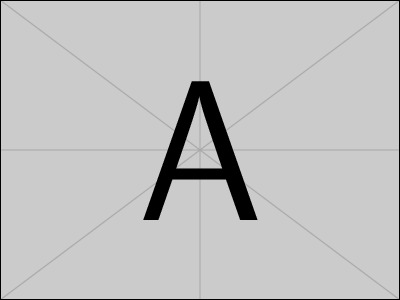
\includegraphics[width=1in]{example-image-a}
  \caption{This test figure tests captions and Table of Contents 
    behavior for very lengthy captions.}
  \label{fig:test2}
\end{figure}

\section{Background}
Test sectioning commands.  We can also have \verb+subsection+, \verb+subsubsection+,
\verb+paragraph+, and \verb+subparagraph+.  Let's try a few:

\subsection{Test Subsection}
\lipsum[1]

\subsection{Another Subsection}
Testing display mathematics:
\begin{equation}
e = mc^2,
\end{equation}
where $e$ is the energy, $m$ is the mass, and the constant $c$ represents the speed of light in a vacuum.

\subsubsection{Subheading}
\lipsum[3-5]
 % Capitulo 1 (editar archivo)
% !TEX root = main.tex
% !TEX encoding = Windows Latin 1
% !TEX TS-program = pdflatex
% 
% Archivo: ch02.tex (Capitulo 2)

\chapter{*******}
\section{*******}




% Fin archivo ch02.tex
\endinput  % Capitulo 2 (editar archivo)
% !TEX root = main.tex
% !TEX encoding = Windows Latin 1
% !TEX TS-program = pdflatex
% 
% Archivo: ch03.tex (Capitulo 3)

\chapter{*******}
\section{*******}




% Fin archivo ch03.tex
\endinput  % Capitulo 3 (editar archivo)
%\include{ch04} % etc...
% Anadir los que sean necesarios.

\appendix % Apendices de la tesis
% !TEX root = main.tex
% !TEX encoding = Windows Latin 1
% !TEX TS-program = pdflatex
% 
% Archivo: ap01.tex (Apendice 1)

\chapter{This Is My First Appendix bla bla bla bla bla bla bla bla}
\section{This Is My First Section bla bla bla bla bla bla bla bla bla bla bla bla }
\noindent
First sentence.\footnote{And this is my first footnote. And this is my first footnote. And this is my first footnote. And this is my first footnote. And this is my first footnote. And this is my first footnote. And this is my first footnote. And this is my first footnote. And this is my first footnote. And this is my first footnote. And this is my first footnote. And this is my first footnote. And this is my first footnote. And this is my first footnote. And this is my first footnote.}\index{Concepto}

\subsection{This Is My First Subsection}
\noindent
% !TEX root = main.tex
% !TEX encoding = Windows Latin 1
% !TEX TS-program = pdflatex
% 
Duis tristique \index{sollicitudin} sollicitudin leo nec consequat. Praesent et dui convallis velit tincidunt fermentum. Mauris cursus purus at sem viverra sed imperdiet sapien imperdiet. Aliquam mattis, elit eget rutrum vulputate, tortor sem pulvinar justo, sit amet mollis felis sem at nibh. Donec malesuada, neque id interdum eleifend, arcu augue porta elit, nec tristique libero metus at massa. Fusce fringilla laoreet rhoncus. Suspendisse potenti. Phasellus dignissim sodales mauris at pharetra. Donec gravida fringilla velit ac rutrum. Curabitur ornare lectus id diam molestie eu imperdiet nulla tempus. Maecenas vestibulum enim et dui ornare blandit. Vivamus \index{fermentum} faucibus viverra. Maecenas at justo sapien. Aenean rhoncus augue mattis purus rhoncus venenatis. Suspendisse metus felis, porttitor in varius in, vulputate at tortor. Aliquam molestie, turpis et malesuada porta, tortor sapien pharetra sapien, ac rhoncus quam dolor a sapien. Pellentesque varius laoreet enim ut auctor. Nullam nec ultricies nisi. Nullam porta lectus et ante consectetur posuere. \cite{texbook} 

%% 
%% Copyright (C) 2014 by Patrick Happel
%% 
%% This file may be distributed and/or modified under the 
%% conditions of the LaTeX Project Public License, either 
%% version 1.2 of this license or (at your option) any later 
%% version. The latest version of this license is in: 
%% 
%% http://www.latex-project.org/lppl.txt 
%% 
%% and version 1.2 or later is part of all distributions of 
%% LaTeX version 1999/12/01 or later.
%%
\input docstrip.tex
\keepsilent
\usedir{tex/latex/lipsum}
\preamble

This is a generated file. 

Copyright (C) 2014 by Patrick Happel 

This file may be distributed and/or modified under the 
conditions of the LaTeX Project Public License, either 
version 1.2 of this license or (at your option) any later
version. The latest version of this license is in:

   http://www.latex-project.org/lppl.txt 

and version 1.2 or later is part of all distributions of 
LaTeX version 1999/12/01 or later. 

\endpreamble

\generate{\file{lipsum.sty}{\from{lipsum.dtx}{package}}}

\obeyspaces
\Msg{****************************************************} 
\Msg{*                                                  *} 
\Msg{* To finish the installation you have to move the  *} 
\Msg{* following file into a directory searched by TeX: *} 
\Msg{*                                                  *} 
\Msg{* lipsum.sty                                       *} 
\Msg{*                                                  *} 
\Msg{* To produce the documentation run the file        *} 
\Msg{* lipsum.dtx through LaTeX.                        *} 
\Msg{*                                                  *} 
\Msg{* Happy TeXing!                                    *} 
\Msg{*                                                  *} 
\Msg{****************************************************}

\endbatchfile


%% 
%% Copyright (C) 2014 by Patrick Happel
%% 
%% This file may be distributed and/or modified under the 
%% conditions of the LaTeX Project Public License, either 
%% version 1.2 of this license or (at your option) any later 
%% version. The latest version of this license is in: 
%% 
%% http://www.latex-project.org/lppl.txt 
%% 
%% and version 1.2 or later is part of all distributions of 
%% LaTeX version 1999/12/01 or later.
%%
\input docstrip.tex
\keepsilent
\usedir{tex/latex/lipsum}
\preamble

This is a generated file. 

Copyright (C) 2014 by Patrick Happel 

This file may be distributed and/or modified under the 
conditions of the LaTeX Project Public License, either 
version 1.2 of this license or (at your option) any later
version. The latest version of this license is in:

   http://www.latex-project.org/lppl.txt 

and version 1.2 or later is part of all distributions of 
LaTeX version 1999/12/01 or later. 

\endpreamble

\generate{\file{lipsum.sty}{\from{lipsum.dtx}{package}}}

\obeyspaces
\Msg{****************************************************} 
\Msg{*                                                  *} 
\Msg{* To finish the installation you have to move the  *} 
\Msg{* following file into a directory searched by TeX: *} 
\Msg{*                                                  *} 
\Msg{* lipsum.sty                                       *} 
\Msg{*                                                  *} 
\Msg{* To produce the documentation run the file        *} 
\Msg{* lipsum.dtx through LaTeX.                        *} 
\Msg{*                                                  *} 
\Msg{* Happy TeXing!                                    *} 
\Msg{*                                                  *} 
\Msg{****************************************************}

\endbatchfile


%% 
%% Copyright (C) 2014 by Patrick Happel
%% 
%% This file may be distributed and/or modified under the 
%% conditions of the LaTeX Project Public License, either 
%% version 1.2 of this license or (at your option) any later 
%% version. The latest version of this license is in: 
%% 
%% http://www.latex-project.org/lppl.txt 
%% 
%% and version 1.2 or later is part of all distributions of 
%% LaTeX version 1999/12/01 or later.
%%
\input docstrip.tex
\keepsilent
\usedir{tex/latex/lipsum}
\preamble

This is a generated file. 

Copyright (C) 2014 by Patrick Happel 

This file may be distributed and/or modified under the 
conditions of the LaTeX Project Public License, either 
version 1.2 of this license or (at your option) any later
version. The latest version of this license is in:

   http://www.latex-project.org/lppl.txt 

and version 1.2 or later is part of all distributions of 
LaTeX version 1999/12/01 or later. 

\endpreamble

\generate{\file{lipsum.sty}{\from{lipsum.dtx}{package}}}

\obeyspaces
\Msg{****************************************************} 
\Msg{*                                                  *} 
\Msg{* To finish the installation you have to move the  *} 
\Msg{* following file into a directory searched by TeX: *} 
\Msg{*                                                  *} 
\Msg{* lipsum.sty                                       *} 
\Msg{*                                                  *} 
\Msg{* To produce the documentation run the file        *} 
\Msg{* lipsum.dtx through LaTeX.                        *} 
\Msg{*                                                  *} 
\Msg{* Happy TeXing!                                    *} 
\Msg{*                                                  *} 
\Msg{****************************************************}

\endbatchfile


\subsubsection{This Is My First Subsubsection}
\noindent
% !TEX root = main.tex
% !TEX encoding = Windows Latin 1
% !TEX TS-program = pdflatex
% 
Duis tristique \index{sollicitudin} sollicitudin leo nec consequat. Praesent et dui convallis velit tincidunt fermentum. Mauris cursus purus at sem viverra sed imperdiet sapien imperdiet. Aliquam mattis, elit eget rutrum vulputate, tortor sem pulvinar justo, sit amet mollis felis sem at nibh. Donec malesuada, neque id interdum eleifend, arcu augue porta elit, nec tristique libero metus at massa. Fusce fringilla laoreet rhoncus. Suspendisse potenti. Phasellus dignissim sodales mauris at pharetra. Donec gravida fringilla velit ac rutrum. Curabitur ornare lectus id diam molestie eu imperdiet nulla tempus. Maecenas vestibulum enim et dui ornare blandit. Vivamus \index{fermentum} faucibus viverra. Maecenas at justo sapien. Aenean rhoncus augue mattis purus rhoncus venenatis. Suspendisse metus felis, porttitor in varius in, vulputate at tortor. Aliquam molestie, turpis et malesuada porta, tortor sapien pharetra sapien, ac rhoncus quam dolor a sapien. Pellentesque varius laoreet enim ut auctor. Nullam nec ultricies nisi. Nullam porta lectus et ante consectetur posuere. \cite{texbook}

%% 
%% Copyright (C) 2014 by Patrick Happel
%% 
%% This file may be distributed and/or modified under the 
%% conditions of the LaTeX Project Public License, either 
%% version 1.2 of this license or (at your option) any later 
%% version. The latest version of this license is in: 
%% 
%% http://www.latex-project.org/lppl.txt 
%% 
%% and version 1.2 or later is part of all distributions of 
%% LaTeX version 1999/12/01 or later.
%%
\input docstrip.tex
\keepsilent
\usedir{tex/latex/lipsum}
\preamble

This is a generated file. 

Copyright (C) 2014 by Patrick Happel 

This file may be distributed and/or modified under the 
conditions of the LaTeX Project Public License, either 
version 1.2 of this license or (at your option) any later
version. The latest version of this license is in:

   http://www.latex-project.org/lppl.txt 

and version 1.2 or later is part of all distributions of 
LaTeX version 1999/12/01 or later. 

\endpreamble

\generate{\file{lipsum.sty}{\from{lipsum.dtx}{package}}}

\obeyspaces
\Msg{****************************************************} 
\Msg{*                                                  *} 
\Msg{* To finish the installation you have to move the  *} 
\Msg{* following file into a directory searched by TeX: *} 
\Msg{*                                                  *} 
\Msg{* lipsum.sty                                       *} 
\Msg{*                                                  *} 
\Msg{* To produce the documentation run the file        *} 
\Msg{* lipsum.dtx through LaTeX.                        *} 
\Msg{*                                                  *} 
\Msg{* Happy TeXing!                                    *} 
\Msg{*                                                  *} 
\Msg{****************************************************}

\endbatchfile


%% 
%% Copyright (C) 2014 by Patrick Happel
%% 
%% This file may be distributed and/or modified under the 
%% conditions of the LaTeX Project Public License, either 
%% version 1.2 of this license or (at your option) any later 
%% version. The latest version of this license is in: 
%% 
%% http://www.latex-project.org/lppl.txt 
%% 
%% and version 1.2 or later is part of all distributions of 
%% LaTeX version 1999/12/01 or later.
%%
\input docstrip.tex
\keepsilent
\usedir{tex/latex/lipsum}
\preamble

This is a generated file. 

Copyright (C) 2014 by Patrick Happel 

This file may be distributed and/or modified under the 
conditions of the LaTeX Project Public License, either 
version 1.2 of this license or (at your option) any later
version. The latest version of this license is in:

   http://www.latex-project.org/lppl.txt 

and version 1.2 or later is part of all distributions of 
LaTeX version 1999/12/01 or later. 

\endpreamble

\generate{\file{lipsum.sty}{\from{lipsum.dtx}{package}}}

\obeyspaces
\Msg{****************************************************} 
\Msg{*                                                  *} 
\Msg{* To finish the installation you have to move the  *} 
\Msg{* following file into a directory searched by TeX: *} 
\Msg{*                                                  *} 
\Msg{* lipsum.sty                                       *} 
\Msg{*                                                  *} 
\Msg{* To produce the documentation run the file        *} 
\Msg{* lipsum.dtx through LaTeX.                        *} 
\Msg{*                                                  *} 
\Msg{* Happy TeXing!                                    *} 
\Msg{*                                                  *} 
\Msg{****************************************************}

\endbatchfile


%% 
%% Copyright (C) 2014 by Patrick Happel
%% 
%% This file may be distributed and/or modified under the 
%% conditions of the LaTeX Project Public License, either 
%% version 1.2 of this license or (at your option) any later 
%% version. The latest version of this license is in: 
%% 
%% http://www.latex-project.org/lppl.txt 
%% 
%% and version 1.2 or later is part of all distributions of 
%% LaTeX version 1999/12/01 or later.
%%
\input docstrip.tex
\keepsilent
\usedir{tex/latex/lipsum}
\preamble

This is a generated file. 

Copyright (C) 2014 by Patrick Happel 

This file may be distributed and/or modified under the 
conditions of the LaTeX Project Public License, either 
version 1.2 of this license or (at your option) any later
version. The latest version of this license is in:

   http://www.latex-project.org/lppl.txt 

and version 1.2 or later is part of all distributions of 
LaTeX version 1999/12/01 or later. 

\endpreamble

\generate{\file{lipsum.sty}{\from{lipsum.dtx}{package}}}

\obeyspaces
\Msg{****************************************************} 
\Msg{*                                                  *} 
\Msg{* To finish the installation you have to move the  *} 
\Msg{* following file into a directory searched by TeX: *} 
\Msg{*                                                  *} 
\Msg{* lipsum.sty                                       *} 
\Msg{*                                                  *} 
\Msg{* To produce the documentation run the file        *} 
\Msg{* lipsum.dtx through LaTeX.                        *} 
\Msg{*                                                  *} 
\Msg{* Happy TeXing!                                    *} 
\Msg{*                                                  *} 
\Msg{****************************************************}

\endbatchfile


\section{This Is My Second Section}
\noindent
% !TEX root = main.tex
% !TEX encoding = Windows Latin 1
% !TEX TS-program = pdflatex
% 
Duis tristique \index{sollicitudin} sollicitudin leo nec consequat. Praesent et dui convallis velit tincidunt fermentum. Mauris cursus purus at sem viverra sed imperdiet sapien imperdiet. Aliquam mattis, elit eget rutrum vulputate, tortor sem pulvinar justo, sit amet mollis felis sem at nibh. Donec malesuada, neque id interdum eleifend, arcu augue porta elit, nec tristique libero metus at massa. Fusce fringilla laoreet rhoncus. Suspendisse potenti. Phasellus dignissim sodales mauris at pharetra. Donec gravida fringilla velit ac rutrum. Curabitur ornare lectus id diam molestie eu imperdiet nulla tempus. Maecenas vestibulum enim et dui ornare blandit. Vivamus \index{fermentum} faucibus viverra. Maecenas at justo sapien. Aenean rhoncus augue mattis purus rhoncus venenatis. Suspendisse metus felis, porttitor in varius in, vulputate at tortor. Aliquam molestie, turpis et malesuada porta, tortor sapien pharetra sapien, ac rhoncus quam dolor a sapien. Pellentesque varius laoreet enim ut auctor. Nullam nec ultricies nisi. Nullam porta lectus et ante consectetur posuere. \footnote{See also \cite{Aup91,Dou72,Hal82}.}


%% 
%% Copyright (C) 2014 by Patrick Happel
%% 
%% This file may be distributed and/or modified under the 
%% conditions of the LaTeX Project Public License, either 
%% version 1.2 of this license or (at your option) any later 
%% version. The latest version of this license is in: 
%% 
%% http://www.latex-project.org/lppl.txt 
%% 
%% and version 1.2 or later is part of all distributions of 
%% LaTeX version 1999/12/01 or later.
%%
\input docstrip.tex
\keepsilent
\usedir{tex/latex/lipsum}
\preamble

This is a generated file. 

Copyright (C) 2014 by Patrick Happel 

This file may be distributed and/or modified under the 
conditions of the LaTeX Project Public License, either 
version 1.2 of this license or (at your option) any later
version. The latest version of this license is in:

   http://www.latex-project.org/lppl.txt 

and version 1.2 or later is part of all distributions of 
LaTeX version 1999/12/01 or later. 

\endpreamble

\generate{\file{lipsum.sty}{\from{lipsum.dtx}{package}}}

\obeyspaces
\Msg{****************************************************} 
\Msg{*                                                  *} 
\Msg{* To finish the installation you have to move the  *} 
\Msg{* following file into a directory searched by TeX: *} 
\Msg{*                                                  *} 
\Msg{* lipsum.sty                                       *} 
\Msg{*                                                  *} 
\Msg{* To produce the documentation run the file        *} 
\Msg{* lipsum.dtx through LaTeX.                        *} 
\Msg{*                                                  *} 
\Msg{* Happy TeXing!                                    *} 
\Msg{*                                                  *} 
\Msg{****************************************************}

\endbatchfile


%% 
%% Copyright (C) 2014 by Patrick Happel
%% 
%% This file may be distributed and/or modified under the 
%% conditions of the LaTeX Project Public License, either 
%% version 1.2 of this license or (at your option) any later 
%% version. The latest version of this license is in: 
%% 
%% http://www.latex-project.org/lppl.txt 
%% 
%% and version 1.2 or later is part of all distributions of 
%% LaTeX version 1999/12/01 or later.
%%
\input docstrip.tex
\keepsilent
\usedir{tex/latex/lipsum}
\preamble

This is a generated file. 

Copyright (C) 2014 by Patrick Happel 

This file may be distributed and/or modified under the 
conditions of the LaTeX Project Public License, either 
version 1.2 of this license or (at your option) any later
version. The latest version of this license is in:

   http://www.latex-project.org/lppl.txt 

and version 1.2 or later is part of all distributions of 
LaTeX version 1999/12/01 or later. 

\endpreamble

\generate{\file{lipsum.sty}{\from{lipsum.dtx}{package}}}

\obeyspaces
\Msg{****************************************************} 
\Msg{*                                                  *} 
\Msg{* To finish the installation you have to move the  *} 
\Msg{* following file into a directory searched by TeX: *} 
\Msg{*                                                  *} 
\Msg{* lipsum.sty                                       *} 
\Msg{*                                                  *} 
\Msg{* To produce the documentation run the file        *} 
\Msg{* lipsum.dtx through LaTeX.                        *} 
\Msg{*                                                  *} 
\Msg{* Happy TeXing!                                    *} 
\Msg{*                                                  *} 
\Msg{****************************************************}

\endbatchfile


%% 
%% Copyright (C) 2014 by Patrick Happel
%% 
%% This file may be distributed and/or modified under the 
%% conditions of the LaTeX Project Public License, either 
%% version 1.2 of this license or (at your option) any later 
%% version. The latest version of this license is in: 
%% 
%% http://www.latex-project.org/lppl.txt 
%% 
%% and version 1.2 or later is part of all distributions of 
%% LaTeX version 1999/12/01 or later.
%%
\input docstrip.tex
\keepsilent
\usedir{tex/latex/lipsum}
\preamble

This is a generated file. 

Copyright (C) 2014 by Patrick Happel 

This file may be distributed and/or modified under the 
conditions of the LaTeX Project Public License, either 
version 1.2 of this license or (at your option) any later
version. The latest version of this license is in:

   http://www.latex-project.org/lppl.txt 

and version 1.2 or later is part of all distributions of 
LaTeX version 1999/12/01 or later. 

\endpreamble

\generate{\file{lipsum.sty}{\from{lipsum.dtx}{package}}}

\obeyspaces
\Msg{****************************************************} 
\Msg{*                                                  *} 
\Msg{* To finish the installation you have to move the  *} 
\Msg{* following file into a directory searched by TeX: *} 
\Msg{*                                                  *} 
\Msg{* lipsum.sty                                       *} 
\Msg{*                                                  *} 
\Msg{* To produce the documentation run the file        *} 
\Msg{* lipsum.dtx through LaTeX.                        *} 
\Msg{*                                                  *} 
\Msg{* Happy TeXing!                                    *} 
\Msg{*                                                  *} 
\Msg{****************************************************}

\endbatchfile


\begin{table}[h]
  \begin{center}
\begin{tabular}{|r|l|}
  \hline
  7C0 & hexadecimal \\
  3700 & octal \\ \cline{2-2}
  11111000000 & binary \\
  \hline \hline
  1984 & decimal \\
  \hline
\end{tabular}
\caption{This is my first table}
\end{center}
\end{table}

\section{This Is My Third Section}
\noindent
% !TEX root = main.tex
% !TEX encoding = Windows Latin 1
% !TEX TS-program = pdflatex
% 
Duis tristique \index{sollicitudin} sollicitudin leo nec consequat. Praesent et dui convallis velit tincidunt fermentum. Mauris cursus purus at sem viverra sed imperdiet sapien imperdiet. Aliquam mattis, elit eget rutrum vulputate, tortor sem pulvinar justo, sit amet mollis felis sem at nibh. Donec malesuada, neque id interdum eleifend, arcu augue porta elit, nec tristique libero metus at massa. Fusce fringilla laoreet rhoncus. Suspendisse potenti. Phasellus dignissim sodales mauris at pharetra. Donec gravida fringilla velit ac rutrum. Curabitur ornare lectus id diam molestie eu imperdiet nulla tempus. Maecenas vestibulum enim et dui ornare blandit. Vivamus \index{fermentum} faucibus viverra. Maecenas at justo sapien. Aenean rhoncus augue mattis purus rhoncus venenatis. Suspendisse metus felis, porttitor in varius in, vulputate at tortor. Aliquam molestie, turpis et malesuada porta, tortor sapien pharetra sapien, ac rhoncus quam dolor a sapien. Pellentesque varius laoreet enim ut auctor. Nullam nec ultricies nisi. Nullam porta lectus et ante consectetur posuere. 
\begin{figure}[h]
  \begin{center}
    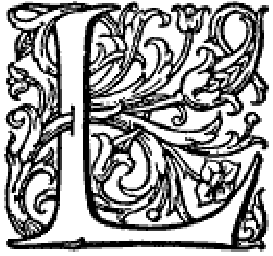
\includegraphics{imagen}
    \caption{This is my first figure}
  \end{center}
\end{figure}


%% 
%% Copyright (C) 2014 by Patrick Happel
%% 
%% This file may be distributed and/or modified under the 
%% conditions of the LaTeX Project Public License, either 
%% version 1.2 of this license or (at your option) any later 
%% version. The latest version of this license is in: 
%% 
%% http://www.latex-project.org/lppl.txt 
%% 
%% and version 1.2 or later is part of all distributions of 
%% LaTeX version 1999/12/01 or later.
%%
\input docstrip.tex
\keepsilent
\usedir{tex/latex/lipsum}
\preamble

This is a generated file. 

Copyright (C) 2014 by Patrick Happel 

This file may be distributed and/or modified under the 
conditions of the LaTeX Project Public License, either 
version 1.2 of this license or (at your option) any later
version. The latest version of this license is in:

   http://www.latex-project.org/lppl.txt 

and version 1.2 or later is part of all distributions of 
LaTeX version 1999/12/01 or later. 

\endpreamble

\generate{\file{lipsum.sty}{\from{lipsum.dtx}{package}}}

\obeyspaces
\Msg{****************************************************} 
\Msg{*                                                  *} 
\Msg{* To finish the installation you have to move the  *} 
\Msg{* following file into a directory searched by TeX: *} 
\Msg{*                                                  *} 
\Msg{* lipsum.sty                                       *} 
\Msg{*                                                  *} 
\Msg{* To produce the documentation run the file        *} 
\Msg{* lipsum.dtx through LaTeX.                        *} 
\Msg{*                                                  *} 
\Msg{* Happy TeXing!                                    *} 
\Msg{*                                                  *} 
\Msg{****************************************************}

\endbatchfile


\begin{figure}[h]
  \begin{center}
    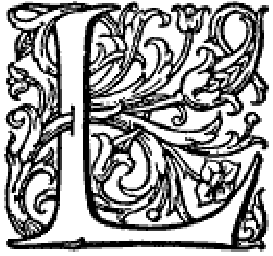
\includegraphics{imagen}
    \caption{This is my second figure}
  \end{center}
\end{figure}

%% 
%% Copyright (C) 2014 by Patrick Happel
%% 
%% This file may be distributed and/or modified under the 
%% conditions of the LaTeX Project Public License, either 
%% version 1.2 of this license or (at your option) any later 
%% version. The latest version of this license is in: 
%% 
%% http://www.latex-project.org/lppl.txt 
%% 
%% and version 1.2 or later is part of all distributions of 
%% LaTeX version 1999/12/01 or later.
%%
\input docstrip.tex
\keepsilent
\usedir{tex/latex/lipsum}
\preamble

This is a generated file. 

Copyright (C) 2014 by Patrick Happel 

This file may be distributed and/or modified under the 
conditions of the LaTeX Project Public License, either 
version 1.2 of this license or (at your option) any later
version. The latest version of this license is in:

   http://www.latex-project.org/lppl.txt 

and version 1.2 or later is part of all distributions of 
LaTeX version 1999/12/01 or later. 

\endpreamble

\generate{\file{lipsum.sty}{\from{lipsum.dtx}{package}}}

\obeyspaces
\Msg{****************************************************} 
\Msg{*                                                  *} 
\Msg{* To finish the installation you have to move the  *} 
\Msg{* following file into a directory searched by TeX: *} 
\Msg{*                                                  *} 
\Msg{* lipsum.sty                                       *} 
\Msg{*                                                  *} 
\Msg{* To produce the documentation run the file        *} 
\Msg{* lipsum.dtx through LaTeX.                        *} 
\Msg{*                                                  *} 
\Msg{* Happy TeXing!                                    *} 
\Msg{*                                                  *} 
\Msg{****************************************************}

\endbatchfile


%% 
%% Copyright (C) 2014 by Patrick Happel
%% 
%% This file may be distributed and/or modified under the 
%% conditions of the LaTeX Project Public License, either 
%% version 1.2 of this license or (at your option) any later 
%% version. The latest version of this license is in: 
%% 
%% http://www.latex-project.org/lppl.txt 
%% 
%% and version 1.2 or later is part of all distributions of 
%% LaTeX version 1999/12/01 or later.
%%
\input docstrip.tex
\keepsilent
\usedir{tex/latex/lipsum}
\preamble

This is a generated file. 

Copyright (C) 2014 by Patrick Happel 

This file may be distributed and/or modified under the 
conditions of the LaTeX Project Public License, either 
version 1.2 of this license or (at your option) any later
version. The latest version of this license is in:

   http://www.latex-project.org/lppl.txt 

and version 1.2 or later is part of all distributions of 
LaTeX version 1999/12/01 or later. 

\endpreamble

\generate{\file{lipsum.sty}{\from{lipsum.dtx}{package}}}

\obeyspaces
\Msg{****************************************************} 
\Msg{*                                                  *} 
\Msg{* To finish the installation you have to move the  *} 
\Msg{* following file into a directory searched by TeX: *} 
\Msg{*                                                  *} 
\Msg{* lipsum.sty                                       *} 
\Msg{*                                                  *} 
\Msg{* To produce the documentation run the file        *} 
\Msg{* lipsum.dtx through LaTeX.                        *} 
\Msg{*                                                  *} 
\Msg{* Happy TeXing!                                    *} 
\Msg{*                                                  *} 
\Msg{****************************************************}

\endbatchfile


%% 
%% Copyright (C) 2014 by Patrick Happel
%% 
%% This file may be distributed and/or modified under the 
%% conditions of the LaTeX Project Public License, either 
%% version 1.2 of this license or (at your option) any later 
%% version. The latest version of this license is in: 
%% 
%% http://www.latex-project.org/lppl.txt 
%% 
%% and version 1.2 or later is part of all distributions of 
%% LaTeX version 1999/12/01 or later.
%%
\input docstrip.tex
\keepsilent
\usedir{tex/latex/lipsum}
\preamble

This is a generated file. 

Copyright (C) 2014 by Patrick Happel 

This file may be distributed and/or modified under the 
conditions of the LaTeX Project Public License, either 
version 1.2 of this license or (at your option) any later
version. The latest version of this license is in:

   http://www.latex-project.org/lppl.txt 

and version 1.2 or later is part of all distributions of 
LaTeX version 1999/12/01 or later. 

\endpreamble

\generate{\file{lipsum.sty}{\from{lipsum.dtx}{package}}}

\obeyspaces
\Msg{****************************************************} 
\Msg{*                                                  *} 
\Msg{* To finish the installation you have to move the  *} 
\Msg{* following file into a directory searched by TeX: *} 
\Msg{*                                                  *} 
\Msg{* lipsum.sty                                       *} 
\Msg{*                                                  *} 
\Msg{* To produce the documentation run the file        *} 
\Msg{* lipsum.dtx through LaTeX.                        *} 
\Msg{*                                                  *} 
\Msg{* Happy TeXing!                                    *} 
\Msg{*                                                  *} 
\Msg{****************************************************}

\endbatchfile


%% 
%% Copyright (C) 2014 by Patrick Happel
%% 
%% This file may be distributed and/or modified under the 
%% conditions of the LaTeX Project Public License, either 
%% version 1.2 of this license or (at your option) any later 
%% version. The latest version of this license is in: 
%% 
%% http://www.latex-project.org/lppl.txt 
%% 
%% and version 1.2 or later is part of all distributions of 
%% LaTeX version 1999/12/01 or later.
%%
\input docstrip.tex
\keepsilent
\usedir{tex/latex/lipsum}
\preamble

This is a generated file. 

Copyright (C) 2014 by Patrick Happel 

This file may be distributed and/or modified under the 
conditions of the LaTeX Project Public License, either 
version 1.2 of this license or (at your option) any later
version. The latest version of this license is in:

   http://www.latex-project.org/lppl.txt 

and version 1.2 or later is part of all distributions of 
LaTeX version 1999/12/01 or later. 

\endpreamble

\generate{\file{lipsum.sty}{\from{lipsum.dtx}{package}}}

\obeyspaces
\Msg{****************************************************} 
\Msg{*                                                  *} 
\Msg{* To finish the installation you have to move the  *} 
\Msg{* following file into a directory searched by TeX: *} 
\Msg{*                                                  *} 
\Msg{* lipsum.sty                                       *} 
\Msg{*                                                  *} 
\Msg{* To produce the documentation run the file        *} 
\Msg{* lipsum.dtx through LaTeX.                        *} 
\Msg{*                                                  *} 
\Msg{* Happy TeXing!                                    *} 
\Msg{*                                                  *} 
\Msg{****************************************************}

\endbatchfile


%% 
%% Copyright (C) 2014 by Patrick Happel
%% 
%% This file may be distributed and/or modified under the 
%% conditions of the LaTeX Project Public License, either 
%% version 1.2 of this license or (at your option) any later 
%% version. The latest version of this license is in: 
%% 
%% http://www.latex-project.org/lppl.txt 
%% 
%% and version 1.2 or later is part of all distributions of 
%% LaTeX version 1999/12/01 or later.
%%
\input docstrip.tex
\keepsilent
\usedir{tex/latex/lipsum}
\preamble

This is a generated file. 

Copyright (C) 2014 by Patrick Happel 

This file may be distributed and/or modified under the 
conditions of the LaTeX Project Public License, either 
version 1.2 of this license or (at your option) any later
version. The latest version of this license is in:

   http://www.latex-project.org/lppl.txt 

and version 1.2 or later is part of all distributions of 
LaTeX version 1999/12/01 or later. 

\endpreamble

\generate{\file{lipsum.sty}{\from{lipsum.dtx}{package}}}

\obeyspaces
\Msg{****************************************************} 
\Msg{*                                                  *} 
\Msg{* To finish the installation you have to move the  *} 
\Msg{* following file into a directory searched by TeX: *} 
\Msg{*                                                  *} 
\Msg{* lipsum.sty                                       *} 
\Msg{*                                                  *} 
\Msg{* To produce the documentation run the file        *} 
\Msg{* lipsum.dtx through LaTeX.                        *} 
\Msg{*                                                  *} 
\Msg{* Happy TeXing!                                    *} 
\Msg{*                                                  *} 
\Msg{****************************************************}

\endbatchfile


% Fin archivo ap01.tex
\endinput  % Apendice 1  (editar archivo)
%\include{ap02} % Apendice 2 (editar archivo)
%\include{ap03} % etc...
% Anadir los que sean necesarios.

%----------------------------------------------------------
\backmatter % Partes finales de la tesis
\renewcommand*{\afterchapskip}{2\onelineskip}

\bibliography{bibliotesis} % Usar el propio o editar este
% (recuerde correr bibtex luego de la primera compilacion)

\CrearIndice % En caso de que haya indice analitico
% (comentar en caso contrario)
% (recuerde correr makeindex luego de la primera compilacion)





\end{document}% ================================================
% end of the main file: main.tex
\typeout{End main.tex}
\endinput